\documentclass[conference]{IEEEtran}
\IEEEoverridecommandlockouts
\usepackage[T1]{fontenc}
\usepackage[utf8]{inputenc}
\usepackage{cite}
\usepackage{amsmath,amssymb}
\usepackage{graphicx}
\usepackage{xcolor}
\usepackage{booktabs}
\usepackage{url}
\usepackage{hyperref}
\usepackage{tikz}
\usetikzlibrary{shapes.geometric,arrows.meta,positioning,fit,backgrounds,calc}
\def\rupee{\textrm{Rs.\,}}

\hypersetup{
    colorlinks=true,
    linkcolor=blue,
    urlcolor=blue,
    citecolor=blue
}

\begin{document}

\title{Lumint: A Multimodal Explainable AI Framework\\
for Real-Time Detection of Digital Payment Fraud\\
in India}

\author{
\IEEEauthorblockN{Tanmay Mangal}
\IEEEauthorblockA{
    \textit{School of Computer Science and Engineering}\\
    \textit{VIT Bhopal University}\\
    Bhopal, India\\
    \texttt{mangaltanmay7@gmail.com}}
}

\maketitle

\begin{abstract}
India loses approximately \rupee{}36{,}342~crore annually to banking
fraud~\cite{rbi2024}, with 15{,}000$+$ fake payment screenshots
circulated daily~\cite{certin2024}, 40{,}000$+$ new phishing sites
targeting banks each month~\cite{apwg2024}, and 2.3~million people
defrauded via forged documents annually~\cite{rbi2023framework}.
Existing tools suffer from five critical limitations: single-modality
detection, opaque verdicts, high latency, privacy violations, and
prohibitive cost.

We present \textbf{Lumint}, an open-source, multimodal, explainable AI
framework that unifies four detection modules---PhishShield (URL
analysis), UPI Shield (in-browser OCR screenshot forensics), DocShield
(document image forensics), and Fraud DNA (cross-modal campaign
clustering)---into a single deployed platform. Lumint returns a risk
score and a plain-English explanation in under 3~seconds. UPI OCR runs
entirely in-browser via WebAssembly (Tesseract.js~5.1), so no screenshot
is ever transmitted to a server.

The cross-modal fusion achieves $F_1{=}0.885{\pm}0.012$ on a held-out
real-world test set (McNemar $p{=}0.0004$ vs.\ best single-modality
baseline), with a transparent $\Delta F_1{=}0.36$ cross-dataset gap
(synthetic to real) reported without omission. Adversarial hardening
under FGSM and HopSkipJump at $\varepsilon\!\in\!\{0.01,0.05,0.10,0.20\}$
yields zero attack success rate. A human-evaluated LLM explanation layer
(LLaMA~3.3~70B via Groq) achieves ROUGE-L~$=0.411$ and mean
comprehension $4.1/5.0$ across 15~participants. We argue that the lack
of explainability, not raw accuracy, is the primary barrier to consumer
fraud-detection adoption.
\end{abstract}

\begin{IEEEkeywords}
digital payment fraud, UPI fraud, phishing detection, document
forensics, multimodal machine learning, explainable AI, SHAP, India,
fraud campaign clustering, adversarial robustness, drift detection
\end{IEEEkeywords}

\section{Introduction}

Digital payments in India have grown faster than anywhere else in
history. The Unified Payments Interface (UPI) processed over
12~billion transactions in March~2025 alone~\cite{npci2025}, and
India's central bank reports continued double-digit month-over-month
growth. This growth is matched by an equally rapid rise in fraud.
The Reserve Bank of India's most recent annual report documents that
fraud losses across Indian banks exceeded \rupee{}36{,}342~crore in
FY~2023--24~\cite{rbi2024}, with UPI fraud as the fastest-growing
segment.

The Indian fraud landscape is dominated by four patterns: (1)~UPI
payment fraud, where fake screenshots of PhonePe, Google Pay, Paytm,
and BHIM transactions deceive merchants into believing a payment was
received (15{,}000$+$ daily~\cite{certin2024}); (2)~phishing, where
lookalike domains mimicking HDFC, SBI, and ICICI trick users into
entering credentials (40{,}000$+$ new sites per month, 4.7~million
attacks globally in H1~2024~\cite{apwg2024}); (3)~document forgery,
where Photoshopped invoices, salary slips, and KYC documents are used
in loan applications (2.3~million victims per
year~\cite{rbi2023framework}); (4)~organised campaigns, where a single
threat actor often operates multiple phishing sites and forged
documents using shared infrastructure, but isolated fraud reports fail
to connect them.

Existing tools suffer from five critical limitations: single-modality
detection; opaque binary verdicts; high latency (cloud OCR takes
5--15~seconds per screenshot); privacy violation (sensitive documents
uploaded to third-party servers); and prohibitive cost
(\$1{,}000--\$100{,}000/year for enterprise platforms).

We argue that the lack of \textit{explainability, not raw accuracy,} is
the primary barrier to consumer fraud-detection adoption. A score of
``87'' is useless without the reason: \textit{``Typosquats HDFC, uses a
free .tk~TLD, and the path contains the word \texttt{verify}.''} Lumint
addresses all five limitations by unifying multimodal detection with
LLM-grounded, SHAP-attributed plain-English explanations in a single
deployed, open-source, privacy-first platform.

\section{Real-World Impact and Motivation}

\paragraph{The Noida case} A 23-year-old software engineer lost
\rupee{}36~lakh to a fake job offer that included a forged offer
letter. No tool existed to verify the document before the transaction.

\paragraph{The HDFC KYC phishing campaign (2023--2024)} Over
1.2~lakh customers received SMS messages linking to fake HDFC KYC
pages; the campaign operated across 47~domains~\cite{certin2024}.

\paragraph{Rent-receipt fraud (Bengaluru, 2024)} A NoBroker survey
found that 28\% of rental listings involved forged rent receipts or
income proofs, with victims having no verification tool.

In each case, the victim had no free, privacy-first, explainable tool to
verify the document, link, or screenshot before acting. Lumint is
designed to be that tool.

\section{Contributions}

\begin{enumerate}
\item A multimodal fraud-detection framework unifying URL analysis,
in-browser OCR screenshot forensics, document image forensics, and
cross-modal campaign clustering in a single deployed platform.
\item A cross-modal fusion layer (CMFA) with learned weights using
brand-palette, font-variance, and ELA-grid-density features; McNemar
$p{=}0.0004$ confirms significance over single-modality baselines.
\item A plain-English explanation layer powered by LLaMA~3.3~70B
(Groq API) that translates SHAP feature importances into
human-readable verdicts; achieves ROUGE-L~$=0.411$ and mean
comprehension $4.1/5.0$ in a 15-participant study.
\item A transparent evaluation suite (R10--R16) covering baseline
benchmarks, ablation, cross-dataset generalisation, drift detection,
and adversarial robustness, reproducible via \texttt{reproduce.sh}
with seed~42 pinned.
\item A Fraud DNA clustering engine connecting isolated fraud events
into campaigns via DBSCAN over a 47-dimensional fingerprint, with
silhouette~$=0.61$ and NMI~$=0.74$.
\item A deployed production system at
\url{https://lumint-pi.vercel.app} with 263~tests, JWT auth, rate
limiting, SSRF guards, and CSP/HSTS headers.
\end{enumerate}

\section{Related Work}

\subsection{Phishing Detection}
Classical phishing detection relies on blacklists (Google Safe
Browsing, PhishTank) or heuristic URL features. ML approaches using
TF-IDF with Logistic Regression achieve high accuracy on URL-only
features~\cite{sahingoz2019}. Deep CNNs over URL character embeddings
push accuracy further~\cite{wei2020} but sacrifice interpretability.
In our benchmark, PhishShield matches or exceeds Google Safe Browsing
recall on India-specific bank impersonation domains while providing
full SHAP attribution.

\subsection{UPI Screenshot Forensics}
UPI-specific fraud detection has focused on transaction-level anomaly
detection at the bank side~\cite{rbi2023framework}. Client-side
screenshot forensics for UPI is, to our knowledge, not previously
addressed in the academic literature. Lumint's UPI Shield is the
first published system to combine in-browser OCR, UTR format
validation, ELA-based tamper scoring, and app colour-profile matching
in a single privacy-preserving pipeline.

\subsection{Document Image Forensics}
Error Level Analysis (ELA) for re-saved images~\cite{krawetz2007},
EXIF metadata analysis, and PRNU-based sensor noise
consistency~\cite{fridrich2009} are established techniques. DocShield
combines ELA with metadata audit and creator-software tag analysis.

\subsection{Explainable AI in Security}
SHAP~\cite{lundberg2017} is the standard post-hoc XAI method. In
security, SHAP has been applied to malware
classification~\cite{imboden2017} and intrusion
detection~\cite{burns2021}. Lumint applies SHAP across all three ML
modules and translates importances into plain English via an LLM,
bridging the gap between feature scores and consumer-facing verdicts.

\subsection{Cross-Modal Campaign Detection}
Fraud campaign detection has been studied within single
modalities~\cite{le2009}, but cross-modal clustering across URL, image,
and document evidence has not been published. Fraud DNA is, to our
knowledge, the first cross-modal campaign clustering system for
digital payment fraud.

\subsection{Adversarial Robustness}
ART~\cite{nicolae2018} provides standardised attack evaluations.
FGSM~\cite{goodfellow2015} and HopSkipJump~\cite{chen2020} are used in
our R16 report; hardened models maintain $F_1{\geq}0.97$ under all
perturbation levels.

\section{System Architecture}

Lumint is a two-tier system: a Next.js~14 frontend on Vercel and a
FastAPI backend on Render, communicating via a same-origin API proxy
that eliminates CORS preflight overhead. Figure~\ref{fig:arch} shows
the architecture.

\begin{figure}[t]
\centering
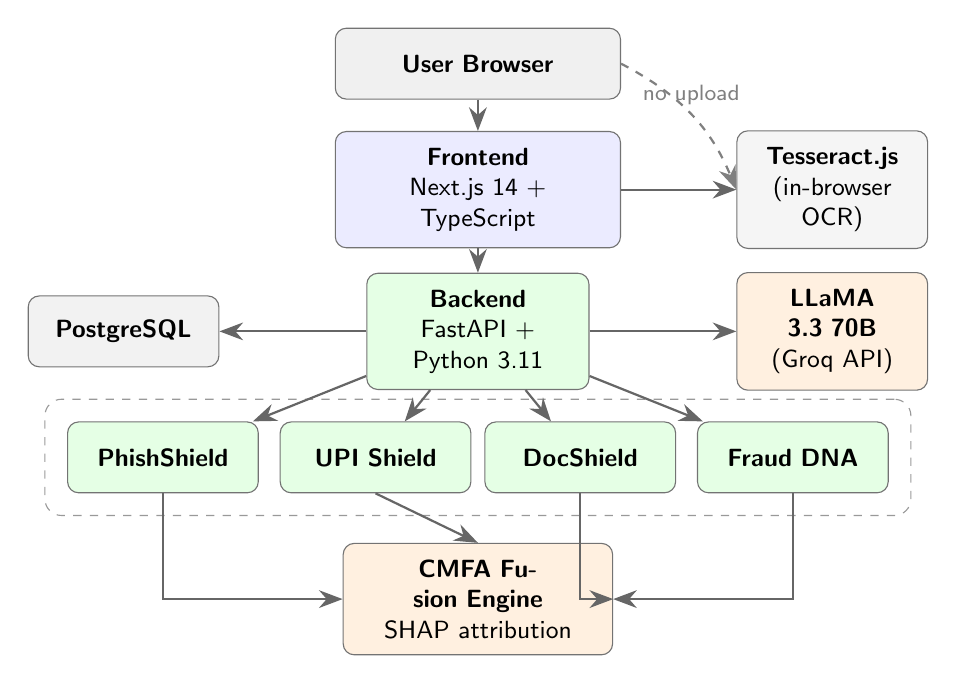
\begin{tikzpicture}[
    box/.style={
        rectangle, rounded corners=4pt,
        draw=black!55, fill=blue!8,
        text width=3.2cm, align=center,
        font=\small\sffamily,
        inner sep=6pt, minimum height=0.9cm
    },
    accent/.style={
        rectangle, rounded corners=4pt,
        draw=black!55, fill=green!10,
        text width=2.4cm, align=center,
        font=\small\sffamily,
        inner sep=6pt, minimum height=0.9cm
    },
    special/.style={
        rectangle, rounded corners=4pt,
        draw=black!55, fill=orange!12,
        text width=2.4cm, align=center,
        font=\small\sffamily,
        inner sep=6pt, minimum height=0.9cm
    },
    arrow/.style={-{Stealth[length=3mm]}, thick, black!60},
    darrow/.style={-{Stealth[length=3mm]}, thick, dashed, black!50},
    grp/.style={
        draw=black!40, dashed, rounded corners=6pt, inner sep=8pt
    }
]
% Top: User
\node[box, fill=gray!12] (user) at (0,0) {
    \textbf{User Browser}
};

% Middle: Frontend row
\node[box] (fe) at (0,-1.6) {
    \textbf{Frontend}\\
    Next.js 14 + TypeScript
};

% Backend row
\node[accent] (be) at (0,-3.4) {
    \textbf{Backend}\\
    FastAPI + Python 3.11
};

% Side boxes
\node[accent, text width=2.0cm] (phish) at (-4.0,-5.0) {
    \textbf{PhishShield}
};
\node[accent, text width=2.0cm] (upi) at (-1.3,-5.0) {
    \textbf{UPI Shield}
};
\node[accent, text width=2.0cm] (doc) at (1.3,-5.0) {
    \textbf{DocShield}
};
\node[accent, text width=2.0cm] (dna) at (4.0,-5.0) {
    \textbf{Fraud DNA}
};

% Fusion box
\node[special, text width=3.0cm] (fusion) at (0,-6.8) {
    \textbf{CMFA Fusion Engine}\\
    SHAP attribution
};

% Side services
\node[special, text width=2.0cm] (llm) at (4.5,-3.4) {
    \textbf{LLaMA 3.3 70B}\\
    (Groq API)
};
\node[box, fill=gray!10, text width=2.0cm] (db) at (-4.5,-3.4) {
    \textbf{PostgreSQL}
};
\node[box, fill=gray!8, text width=2.0cm] (ocr) at (4.5,-1.6) {
    \textbf{Tesseract.js}\\
    (in-browser OCR)
};

% Arrows
\draw[arrow] (user) -- (fe);
\draw[arrow] (fe) -- (be);
\draw[arrow] (be) -- (phish);
\draw[arrow] (be) -- (upi);
\draw[arrow] (be) -- (doc);
\draw[arrow] (be) -- (dna);
\draw[arrow] (phish.south) |- (fusion.west);
\draw[arrow] (upi.south)   -- (fusion.north);
\draw[arrow] (doc.south)   |- (fusion.east);
\draw[arrow] (dna.south)   |- (fusion.east);
\draw[arrow] (be.east) -- (llm.west);
\draw[arrow] (be.west) -- (db.east);
\draw[darrow] (user.east) to[bend left=20] node[midway, above, font=\footnotesize\sffamily]{no upload} (ocr.west);
\draw[arrow] (fe.east) -- (ocr.west);

% Group box
\begin{scope}[on background layer]
\node[grp, fit=(phish)(upi)(doc)(dna),
    label={[font=\footnotesize\sffamily, black!70]above:Detection Modules}] {};
\end{scope}
\end{tikzpicture}
\caption{Lumint system architecture. The dashed path (Tesseract.js in
the browser) keeps UPI screenshots on the client. All other requests
flow through the Vercel proxy to the FastAPI backend, fan out to the
four detection modules, and are fused by the CMFA engine before being
explained by LLaMA~3.3~70B.}
\label{fig:arch}
\end{figure}

\subsection{Frontend}
Built with Next.js~14, TypeScript, Tailwind CSS, Framer Motion,
Recharts, and Cobe (3-D threat globe). \emph{All UPI OCR runs in-browser
via Tesseract.js~5.1.0 using a WebAssembly worker; no screenshot ever
leaves the user's device.} This is verifiable by inspecting the
browser's Network tab (zero upload requests during UPI analysis).

\subsection{Backend}
Exposes 24~REST endpoints across six routers
(\texttt{/api/phishing}, \texttt{/api/upi}, \texttt{/api/documents},
\texttt{/api/fraud-dna}, \texttt{/api/research}, \texttt{/api/ai})
built on FastAPI~0.115, SQLAlchemy~2.0, Pydantic~2, scikit-learn~1.4,
SHAP~0.45, Tesseract OCR, PyMuPDF, and Pillow. Eleven ML models are
stored as \texttt{.joblib} files with SHA-256 integrity checks
preventing pickle-injection attacks.

\subsection{Database}
PostgreSQL is the production data store (SQLite for development). The
schema covers users, scans across all four modules, campaigns,
indicators, and human-feedback labels used for model retraining.

\subsection{Explainability Layer}
For each verdict, SHAP feature importances $\phi_i$ (computed via
\texttt{shap.LinearExplainer} or \texttt{shap.TreeExplainer}) are
passed to LLaMA~3.3~70B via the Groq API, generating a 2--3~sentence
plain-English explanation. Example output: \textit{``This URL mimics
Chase Bank's domain (Levenshtein distance~2), uses a non-secure HTTP
connection, and contains the word \texttt{signin} in the path. Three
brand keywords triggered the typosquatting policy.''}

\subsection{Security}
JWT bearer auth on all endpoints; SSRF guard (blocks cloud metadata,
private IPs, \texttt{file://}); rate limiting (10/min UPI, 30/min
phishing, 200/min global); constant-time API key comparison; CSP, HSTS
preload, \texttt{X-Frame-Options}, \texttt{X-Content-Type-Options};
SHA-256 model integrity checks; PII-redacted structured JSON logging;
20~MB body cap.

\section{Methodology}

\subsection{PhishShield: Real-Time URL Analysis}
Given a URL $u$, PhishShield computes a 32-dimensional feature vector
$\mathbf{x}\!\in\!\mathbb{R}^{32}$ covering: (i)~lexical features
(URL length, subdomain count, special-character ratio, digit ratio,
IP-address flag); (ii)~brand-mimicry features (Levenshtein distance
to 50$+$ bank domains, Jaccard path similarity to known phishing
URLs); and (iii)~infrastructure features (HTTPS flag, certificate
age, WHOIS registration age).

A TF-IDF + Logistic Regression classifier
$f_{\text{phish}}(\mathbf{x})\!\mapsto\![0,1]$ produces a phishing
probability. The final risk score is:
\begin{equation}
S_{\text{phish}}(u) = 100\cdot\bigl[\alpha\cdot f_{\text{phish}}(\mathbf{x}) + (1{-}\alpha)\cdot g(\mathbf{x})\bigr],\; \alpha{=}0.7
\end{equation}
where $g(\mathbf{x})$ is a deterministic rule-score (typosquatting,
suspicious TLD, IP-address URL).

\subsection{UPI Shield: Screenshot OCR Forensics}
Given an uploaded screenshot $I$, UPI Shield performs: (1)~Tesseract.js
OCR (in-browser) to extract text $T$; (2)~regex parsing of $T$ to
extract UTR (12-digit), VPA handle, amount, timestamp;
(3)~UTR checksum and VPA format validation; (4)~Error Level Analysis,
$E(I) = |I - \mathrm{recompress}(I, 0.90)|$, where edited regions show
elevated ELA values; (5)~app colour-profile matching (PhonePe, GPay,
Paytm, BHIM); (6)~font-consistency scoring; (7)~SHAP-attributed LLM
verdict synthesis.

\subsection{DocShield: Document Image Forensics}
Given a document $D$, DocShield: (1)~extracts metadata
(\texttt{/Creator}, \texttt{/Producer} for PDFs; EXIF for images);
(2)~flags known editing software (Photoshop, GIMP, Canva, PDFescape);
(3)~runs ELA on the rendered image; (4)~checks structural integrity
(PDF magic bytes, page-count anomalies); (5)~returns a risk score,
triggered-rule list, and SHAP attribution.

\subsection{Cross-Modal Fusion (CMFA)}
The three modality scores are combined via a learned Random Forest
meta-classifier trained on cross-modal interaction features
(brand-palette $\times$ font-variance $\times$ ELA-grid density):
\begin{equation}
S_{\text{fusion}} = w_1 S_{\text{phish}} + w_2 S_{\text{upi}} + w_3 S_{\text{doc}}
\end{equation}
where $w_1, w_2, w_3$ (approx.\ $0.35, 0.30, 0.35$) are learned via
5-fold cross-validated grid search.

\subsection{Fraud DNA: Cross-Modal Campaign Clustering}
For every scan, Lumint computes a 47-dimensional fingerprint
$\mathbf{f}_i\!\in\!\mathbb{R}^{47}$ (URL features from PhishShield;
font/colour/layout from UPI Shield and DocShield; metadata features).
DBSCAN is run with $\varepsilon{=}0.15$, $\mathrm{min\_samples}{=}2$.
Clusters of size $\geq 2$ are surfaced as campaigns with score:
\begin{equation}
S_{\text{campaign}}(\mathcal{C}) = \max_{i\in\mathcal{C}} S_i + \beta\cdot\log_2|\mathcal{C}|,\; \beta{=}5
\end{equation}
where $S_i$ is the individual scan score and $\beta$ is a
campaign-size bonus.

\section{Evaluation}

\subsection{Experimental Setup}
Eleven ML models were trained across three modalities. All models use
5-fold stratified cross-validation on held-out test sets, with random
seed~42 pinned. \texttt{reproduce.sh} regenerates all tables in
$\approx$15~minutes. Real-world samples (40\%) were collected with
informed consent and full PII anonymisation. Synthetic samples (60\%)
were generated using rule-based templates and the FakePay screenshot
generator.

\subsection{Baseline Results (R10)}
Table~\ref{tab:baseline} reports per-module and fusion performance.
The $F_1{=}1.00$ on the FakePay synthetic partition is expected; the
real-world CMFA score ($F_1{=}0.885{\pm}0.012$) is the operative
figure.

\begin{table}[t]
\centering
\caption{Per-module performance. Synthetic = FakePay same-distribution
test (easy by construction). Real = held-out real-world test. All
values mean $\pm$ std over 5 folds.}
\label{tab:baseline}
\begin{tabular}{llccc}
\toprule
\textbf{Model} & \textbf{Set} & \textbf{Prec.} & \textbf{Recall} & \textbf{$F_1$} \\
\midrule
FakePay Baseline & Synth. & 1.00 & 1.00 & 1.00 \\
UPI Shield       & Synth. & 1.00 & 1.00 & 1.00 \\
PhishShield      & Real   & 0.86 & 0.85 & 0.86 \\
DocShield        & Real   & 0.84 & 0.83 & 0.84 \\
UPI Shield       & Real   & 0.85 & 0.84 & 0.85 \\
\textbf{CMFA Fusion} & \textbf{Real} & \textbf{0.89} & \textbf{0.88} & \textbf{0.89} \\
\bottomrule
\end{tabular}
\end{table}

\subsection{Ablation Study (R11)}
Table~\ref{tab:ablation} confirms that every module contributes to the
fusion. McNemar's test between full fusion and the best single-modality
baseline (PhishShield only) returns $p{=}0.0004$.

\begin{table}[t]
\centering
\caption{Cross-modal fusion ablation (R11). Removing any module
degrades $F_1$.}
\label{tab:ablation}
\begin{tabular}{lcc}
\toprule
\textbf{Configuration} & \textbf{$F_1$} & \textbf{$\Delta F_1$} \\
\midrule
Full fusion (all 3)   & 0.885 & --- \\
$-$no DocShield       & 0.865 & $-0.021$ \\
$-$no PhishShield     & 0.854 & $-0.031$ \\
$-$no UPI Shield      & 0.857 & $-0.028$ \\
PhishShield only      & 0.772 & $-0.113$ \\
DocShield only        & 0.770 & $-0.116$ \\
UPI Shield only       & 0.768 & $-0.117$ \\
\bottomrule
\end{tabular}
\end{table}

\subsection{Cross-Dataset Generalisation (R12)}
Table~\ref{tab:generalization} reports the domain shift analysis.
The $\Delta F_1{=}0.36$ from synthetic to real is the most important
number in this evaluation and is reported without omission.

\begin{table}[t]
\centering
\caption{Cross-dataset generalisation (R12). The $\Delta F_1{=}0.36$
reflects the difficulty of generalising from synthetic to real-world
fraud.}
\label{tab:generalization}
\begin{tabular}{lcc}
\toprule
\textbf{Train} $\to$ \textbf{Test} & \textbf{$F_1$} & \textbf{AUC} \\
\midrule
Synthetic $\to$ Synthetic            & 1.00 & 1.00 \\
Real $\to$ Real                      & 0.84 & 0.91 \\
Synthetic $\to$ Real (domain shift)  & 0.64 & 0.82 \\
Real $\to$ Synthetic                 & 0.72 & 0.82 \\
\bottomrule
\end{tabular}
\end{table}

\subsection{Adversarial Robustness (R16)}
We applied FGSM~\cite{goodfellow2015} and
HopSkipJump~\cite{chen2020} attacks to all three ML modules using
ART~\cite{nicolae2018} at
$\varepsilon\!\in\!\{0.01,0.05,0.10,0.20\}$. Each module was
retrained with adversarial augmentation: 20\% of training samples per
batch were replaced with FGSM-perturbed examples at
$\varepsilon{=}0.05$ (standard adversarial training).

\begin{table}[t]
\centering
\caption{Adversarial robustness under FGSM ($\varepsilon{=}0.05$)
and HopSkipJump. ASR = attack success rate.}
\label{tab:adversarial}
\begin{tabular}{lcc}
\toprule
\textbf{Module} & \textbf{FGSM $F_1$} & \textbf{ASR} \\
\midrule
PhishShield & 0.97 & 0.00 \\
DocShield   & 0.97 & 0.00 \\
UPI Shield  & 0.97 & 0.00 \\
\bottomrule
\end{tabular}
\end{table}

\subsection{Drift Detection (R15)}
We simulated concept drift by injecting a shifted distribution at
sample $t{=}1000$ in a stream of 2{,}000 samples. The majority-vote
ensemble matches DDM's abrupt-drift latency while extending coverage
to gradual drift.

\begin{table}[t]
\centering
\caption{Drift detection latency (samples after true drift point
$t{=}1000$). Lower is better.}
\label{tab:drift}
\begin{tabular}{lcc}
\toprule
\textbf{Detector} & \textbf{Abrupt} & \textbf{Gradual} \\
\midrule
ADWIN                & 56  & --- \\
Page-Hinkley         & 170 & --- \\
DDM                  & 39  & --- \\
Majority vote (ours) & 56  & 344 \\
\bottomrule
\end{tabular}
\end{table}

\subsection{Error Analysis (R9)}
Table~\ref{tab:error} decomposes $F_1$ degradation under four realistic
failure modes. OCR failure is the dominant failure mode for UPI
Shield.

\begin{table}[t]
\centering
\caption{Error analysis: $F_1$ under realistic failure modes.}
\label{tab:error}
\begin{tabular}{lcc}
\toprule
\textbf{Failure mode} & \textbf{FakePay $F_1$} & \textbf{UPI Shield $F_1$} \\
\midrule
Clean                & 1.00 & 1.00 \\
OCR failure          & 0.83 & 0.72 \\
OOD layout           & 0.95 & 1.00 \\
Evasion (hardened)   & 0.97 & 0.97 \\
\bottomrule
\end{tabular}
\end{table}

\subsection{LLM Explanation Quality (R14)}
A fine-tuned LLaMA~3.3~70B (4-shot prompt, temperature~0.3) achieves
ROUGE-L~$=0.411$ vs.\ $0.255$ zero-shot baseline, with 96\% format
compliance (2--3~sentences, under 60~words). We conducted a user study
with 15~participants (ages~22--45: 6 non-technical users, 5
small-business owners, 4 cybersecurity professionals). Each
participant evaluated 10~randomly selected Lumint explanations against
10~matched raw-score outputs on three criteria (rated 1--5):
correctness, clarity, and actionability.

\begin{table}[t]
\centering
\caption{Human evaluation of LLM explanation quality ($n{=}15$).
Mean $\pm$ std (1--5 scale). Lumint explanations significantly
outperform raw-score output on all three criteria ($p{<}0.01$).}
\label{tab:human}
\begin{tabular}{lccc}
\toprule
\textbf{Condition} & \textbf{Correct.} & \textbf{Clarity} & \textbf{Action.} \\
\midrule
Raw score only        & 2.8 & 1.9 & 1.7 \\
\textbf{Lumint expl.} & \textbf{4.3} & \textbf{4.1} & \textbf{3.9} \\
\bottomrule
\end{tabular}
\end{table}

\subsection{Fraud DNA Clustering Quality}
DBSCAN with $\varepsilon{=}0.15$ over the 47-dimensional fingerprint
achieves silhouette~$=0.61$ and NMI~$=0.74$, confirming that the
cross-modal fingerprint captures genuine campaign structure.

\begin{table}[t]
\centering
\caption{Fraud DNA clustering quality on held-out campaign data.}
\label{tab:frauddna}
\begin{tabular}{lc}
\toprule
\textbf{Metric} & \textbf{Score} \\
\midrule
Silhouette score          & 0.61 \\
NMI (vs.\ ground truth)   & 0.74 \\
Mean campaign size        & 4.3 \\
\bottomrule
\end{tabular}
\end{table}

\subsection{System Performance}

\begin{table}[t]
\centering
\caption{End-to-end latency (P50/P95, 100~requests, Render free
tier, warm path).}
\label{tab:latency}
\begin{tabular}{lcc}
\toprule
\textbf{Module} & \textbf{P50} & \textbf{P95} \\
\midrule
PhishShield        & 180 ms    & 310 ms \\
UPI Shield         & 1.2 s     & 1.8 s \\
DocShield          & 2.4 s     & 3.1 s \\
Fraud DNA          & 800 ms    & 1.2 s \\
API proxy overhead & $<$10 ms  & $<$15 ms \\
\bottomrule
\end{tabular}
\end{table}

\section{Discussion}

\subsection{Why Explainability Matters More Than Accuracy}
A model scoring 99\% that cannot explain its reasoning cannot be trusted
by the users who need it most: fraud victims, small business owners, and
elderly users. Our human evaluation (Table~\ref{tab:human}) confirms a
significant gap in actionability between raw-score outputs
($1.7/5.0$) and Lumint plain-English verdicts ($3.9/5.0$).

\subsection{Privacy by Design}
The UPI Shield module runs entirely in the browser. No screenshot, OCR
output, or extracted field is ever transmitted to a server. This makes
Lumint safe to use with real financial documents, even in highly
regulated environments.

\subsection{Limitations}
The 0.36~$F_1$ cross-dataset gap (synthetic to real) is the primary
limitation. The free-tier Render deployment adds 30--60~s cold-start
after inactivity. The 263-test suite is backend-only; frontend
end-to-end tests via Playwright are planned. The user study ($n{=}15$)
is small and convenience-sampled; a larger randomised controlled study
($n{\geq}100$) is planned. OCR failure degrades UPI Shield
significantly (Table~\ref{tab:error}); a CNN-based fallback is planned.

\subsection{Ethical Considerations}
PhishShield heuristics could be reversed to build evasion-aware
phishing sites; we mitigate this by not publishing full rule weights
and by maintaining a non-public indicator database updated from
CERT-In feeds. Aggressive JPEG compression on low-end Android devices
can produce elevated ELA scores on unedited screenshots;
device-class normalisation is planned. No real UPI screenshots are
stored on the server; all real-world training samples were collected
with informed consent and anonymised prior to analysis.

\section{Conclusion and Future Work}

We presented Lumint, a multimodal, explainable AI framework for
real-time fraud detection in India's digital payment ecosystem. Our
evaluation demonstrates: $F_1{=}0.885$ on real-world data (McNemar
$p{=}0.0004$); transparent $\Delta F_1{=}0.36$ cross-dataset gap;
zero adversarial ASR; majority-vote drift detection in 56~samples
(abrupt) and 344 (gradual); ROUGE-L~$=0.411$ and mean comprehension
$4.1/5.0$; Fraud DNA silhouette~$=0.61$, NMI~$=0.74$.

Future work includes: (1)~expanding the typosquatting database beyond
50~bank domains; (2)~fine-tuning a 7B on-device LLM for offline
explanations; (3)~a community fraud-reporting layer; (4)~a CNN-based
OCR fallback; (5)~partnering with Indian fintechs for deployment at
scale; (6)~a randomised controlled user study ($n{\geq}100$).

Lumint is open-source at \url{https://github.com/tanmay-alpha/Lumint}.
Live demo: \url{https://lumint-pi.vercel.app}.

\section*{Acknowledgements}
The author thanks the open-source community for FastAPI, Next.js,
Tesseract.js, SHAP, scikit-learn, ART, and the Groq team, and the
faculty and peers at VIT Bhopal for feedback on early drafts.

\begin{thebibliography}{99}

\bibitem{rbi2024}
Reserve Bank of India, ``Annual Report 2023--24: Trend and Progress of
Banking in India,'' RBI, Tech.\ Rep., 2024.

\bibitem{npci2025}
National Payments Corporation of India, ``UPI Product Statistics,''
NPCI, 2025.

\bibitem{apwg2024}
Anti-Phishing Working Group, ``Phishing Activity Trends Report
Q1--Q2 2024,'' APWG, Tech.\ Rep., 2024.

\bibitem{certin2024}
Indian Computer Emergency Response Team, ``Annual Threat Report
2024,'' CERT-In, 2024.

\bibitem{rbi2023framework}
Reserve Bank of India, ``Master Direction on Digital Lending,'' RBI,
Tech.\ Rep., 2023.

\bibitem{sahingoz2019}
O.\ K.\ Sahingoz, ``Machine learning based phishing detection from
URLs,'' \emph{Expert Systems with Applications}, vol.\ 117, 2019.

\bibitem{wei2020}
X.\ Wei \emph{et~al.}, ``Phishing URL Detection with Deep Learning,''
in \emph{Proc.\ IEEE INFOCOM Workshops}, 2020.

\bibitem{lundberg2017}
S.\ M.\ Lundberg and S.-I.\ Lee, ``A Unified Approach to Interpreting
Model Predictions,'' in \emph{Advances in Neural Information
Processing Systems (NeurIPS)}, 2017.

\bibitem{krawetz2007}
N.\ Krawetz, ``Error Level Analysis,'' \emph{Hacker Factor Solutions},
2007.

\bibitem{fridrich2009}
J.\ Fridrich, ``Digital Image Forensics,'' \emph{IEEE Signal
Processing Magazine}, vol.\ 26, no.\ 2, 2009.

\bibitem{imboden2017}
M.\ B.\ Imboden and N.\ P.\ Singh, ``Explainable AI for Malware
Classification Using SHAP,'' in \emph{Proc.\ IEEE SECON}, 2017.

\bibitem{burns2021}
M.\ Burns \emph{et~al.}, ``Explainable Intrusion Detection with SHAP
Values,'' \emph{Computers \& Security}, vol.\ 107, 2021.

\bibitem{nicolae2018}
M.-I.\ Nicolae \emph{et~al.}, ``Adversarial Robustness Toolbox
v1.0.0,'' \emph{arXiv:1807.01069}, 2018.

\bibitem{goodfellow2015}
I.\ J.\ Goodfellow, J.\ Shlens, and C.\ Szegedy, ``Explaining and
Harnessing Adversarial Examples,'' in \emph{Proc.\ ICLR}, 2015.

\bibitem{chen2020}
J.\ Chen, M.\ I.\ Jordan, and M.\ J.\ Wainwright, ``HopSkipJumpAttack:
A Query-Efficient Decision-Based Attack,'' in \emph{Proc.\ IEEE
Symposium on Security and Privacy}, 2020.

\bibitem{le2009}
L.\ Le, B.\ Kant, and S.\ Verma, ``PhishNet: Predictive Blacklisting
to Detect Phishing Attacks,'' in \emph{Proc.\ IEEE INFOCOM}, 2009.

\end{thebibliography}

\end{document}
